\chapter{Data acquisition software}
\label{chapter:dqm4hep}

\epigraph{Before software can be reusable \\it first has to be usable.}{Ralph Johnson}

Data acquisition is a critical component of all modern particle physics experiments across all stages of technological readiness, from the very beginning of hardware testing in tabletop experiments to full-scale international experiments like the Large Hadron Collider. 

In the modern era of particle physics, the interplay of hardware and software at minscule timescales drives everything, and almost all results are highly dependent upon the speed and efficiency of the electronics and computer systems that extract data from the detectors. A massive quantity of work goes into creating, testing and optimising the systems that will acquire, process, sort and transport data before it is ever seen by the physicist operating the experiment.

Of particular interest in this thesis is the data acquisition software during the development phase, where individual detector subcomponents are undergoing prototyping and testing. These development and iteration cycles are tied closely to testbeam facillities such as the \acrfull{SPS} at CERN and the DESY II synchrotron at DESY. At this point in the development cycle, the detectors are beginning to take shape and this is where data acquisition (or \acrshort{DAQ}) becomes an important consideration. 

In addition to this, the data acquisition solutions used during the testbeam phase of detector development is likely to inform the final data acquisition solution; either by evolving directly into the final software, or by identifying and evaluating the particular features or challenges of the subdetector components that the software must take into account or accommodate.

During this stage, each individual detector component -- such as a vertex tracker or hadronic calorimeter -- will be developed by small teams, and the natural tendency is for each of these groups to set their own standards and develop their own tools, prioritising the features that are important to their specific case. However, in the past this approach has generated a variety of \textit{ad hoc} solutions for testbeam software, many of which cannot be applied outside of their original scope. This results in different teams solving the same problems and implementing the same solutions for each subdetector.

An alternative to this is to develop a suite of tools or frameworks that are generic -- capable of being used and deployed for a wide variety of different uses and detector types. In this way, we could greatly reduce the effort used to recreate the same solutions for each new detector, allowing more science to be done faster.

\subsection*{Online monitoring and data quality monitoring}
The area of this that we have chosen to contribute to is the development of online monitoring and data quality monitoring tools. Data from testbeams is often not processed fully until well after it has been taken, sometimes after the testbeam has ended, due to contraints on time or processing power. If there were errors, incongruencies, or any other issues with the data, these issues cannot be identified immediately, and as a result may be present in multiple runs, spoiling data and wasting precious time during the already extremely time-sensitive environment of a testbeam.

Online monitoring addresses these issues by allowing the experimenters to see a ``preview'' of the data being collected. It can provide both a quantitative and qualitative look into how the detectors are responding, and what the data willl look like when properly processed, allowing any potential issues to be identified and fixed in a timely manner. This means that good online monitoring can improve the efficiency of a testbeam, increasing the ``yield'' of data from a given experiment.

Another aspect of this is data quality monitoring (\acrshort{DQM}), which assesses the `quality' of the data being taken. The definition of data's `quality' will vary depending on the hardware, software, and goals of the experiment, but will usually constitute a some from of statistical measure. In this regard, data quality monitoring can be seen as an extension of the concept of online monitoring, focusing more closely on the quantitative aspects. In general, DQM provides the most benefit in more mature experiments, relying on previous experience with the detector and collected data to understand how the data appears when the device is functioning correctly.  

In pursuit of all of the above aims, this chapter will discuss the \acrlong{DQM4hep} tool (\acrshort{DQM4hep}) developed for online monitoring and data quality monitoring, going into detail on its properties, principles, applications and development. Deployment and usage of the framework will be discussed in greater detail in Chapters \ref{chapter:aidatestbeams} and \ref{chapter:ideatestbeam}.

\subsection*{The AIDA-2020 project}
This work on DQM4hep takes place within the context of the AIDA-2020 project, an EU-funded research programme for developing infrastructure and technologies for particle physics detector development and testing, comprising 24 member countries and lead by CERN.

The overarching goal of AIDA-2020 is to develop common tools and infrastructures for physics testbeams. The collaboration is split into work packages focusing on specific areas, and the work detailed in this thesis takes place within Work Package 5 for data acquisition systems for beam tests % Cite AIDA-2020 here 

The goal of this work package is to create a suite of tools that are designed with a variety of possible uses in mind, thereby reducing the work and development time necessary to implement data acquisition and monitoring setups, speeding up the planning and deployment of physics testbeams. 

\section{Overview of DQM4hep}
Data Quality Monitoring for High-Energy Physics (abbreviated DQM4hep) is an online monitoring and data quality monitoring framework developed for physics testbeams for high-energy and particle physics, developed by R\'{e}mi Et\'{e} and Antoine Pingault. It is designed to be able to fulfil the requirements of monitoring for physics testbeams in a generic way. The framework is written in the C++11 standard and can run on any Linux distribution. The only requirements for installation are a compiler compliant with the C++11 standard, cmake 3.4 or higher, and ROOT 6. All other dependencies are downloaded and compiled automatically during installation. 

The two core principles of DQM4hep are genericity and modularity. The framework is based upon a plugin system that allows shared libraries to be loaded and hook classes for further use \cite{aida2020-milestone-dqm4hep}. This structure allows for independent components of the framework to be used, not used, or exchanged, by isolating each function of the program into independent processes. The components that are specific to any particular use case are written by the users, and the rest of the framework then handles packaging this information in a useful way and networking to transmit it to where it is needed, meaning that the user does not have to worry about the mechanics of data storage, serialisation or transmission. 

The experiment-specific components have to be written by the user, but these components use standard C++ code with a few DQM4hep-specific functions to handle their integration into the framework, making them easy to understand for users who already have experience coding in C++. This also means that the framework is capable of working with any data format that can packed into, decoded from, and accessed with normal C++ methods, including those that can be loaded from external libraries. This results in a framework that is able to deal with any kind of data, including user-defined data types, making it more flexible, portable and easily reusable.

\subsection{Architecture}
DQM4hep is designed with genericness as its core paradigm, using processes and algorithms that are independent of data type. The ability to run multiple instances of each process of the framework is also key to its flexibility, allowing users to, for example, separate sub-detector data from data that has undergone event building, operate in online or offline modes, or distribute the computational load of the analysis over several networked computers.

The generic nature of the framework lies in two core features:
\begin{itemize}
	\item The Event Data Model abstraction allows the user to define the type and structure of an event and how serialisation should be handled.
	\item The plugin system allows the inclusion of any user-defined classes via external libraries, such as to select the serialisation process, online analysis, etc.
\end{itemize}

The plugin system for end-users consists of four different types of plugins: analysis modules, standalone modules, file reader plugins, and file streamer plugins. Each of these will be discussed in-depth in the sections below.

A diagrammatical representation of the overall structure of the framework can be seen in Fig. \ref{figure:daq/dqm4hep/architecture}.

\begin{figure}[p]
	\centering
	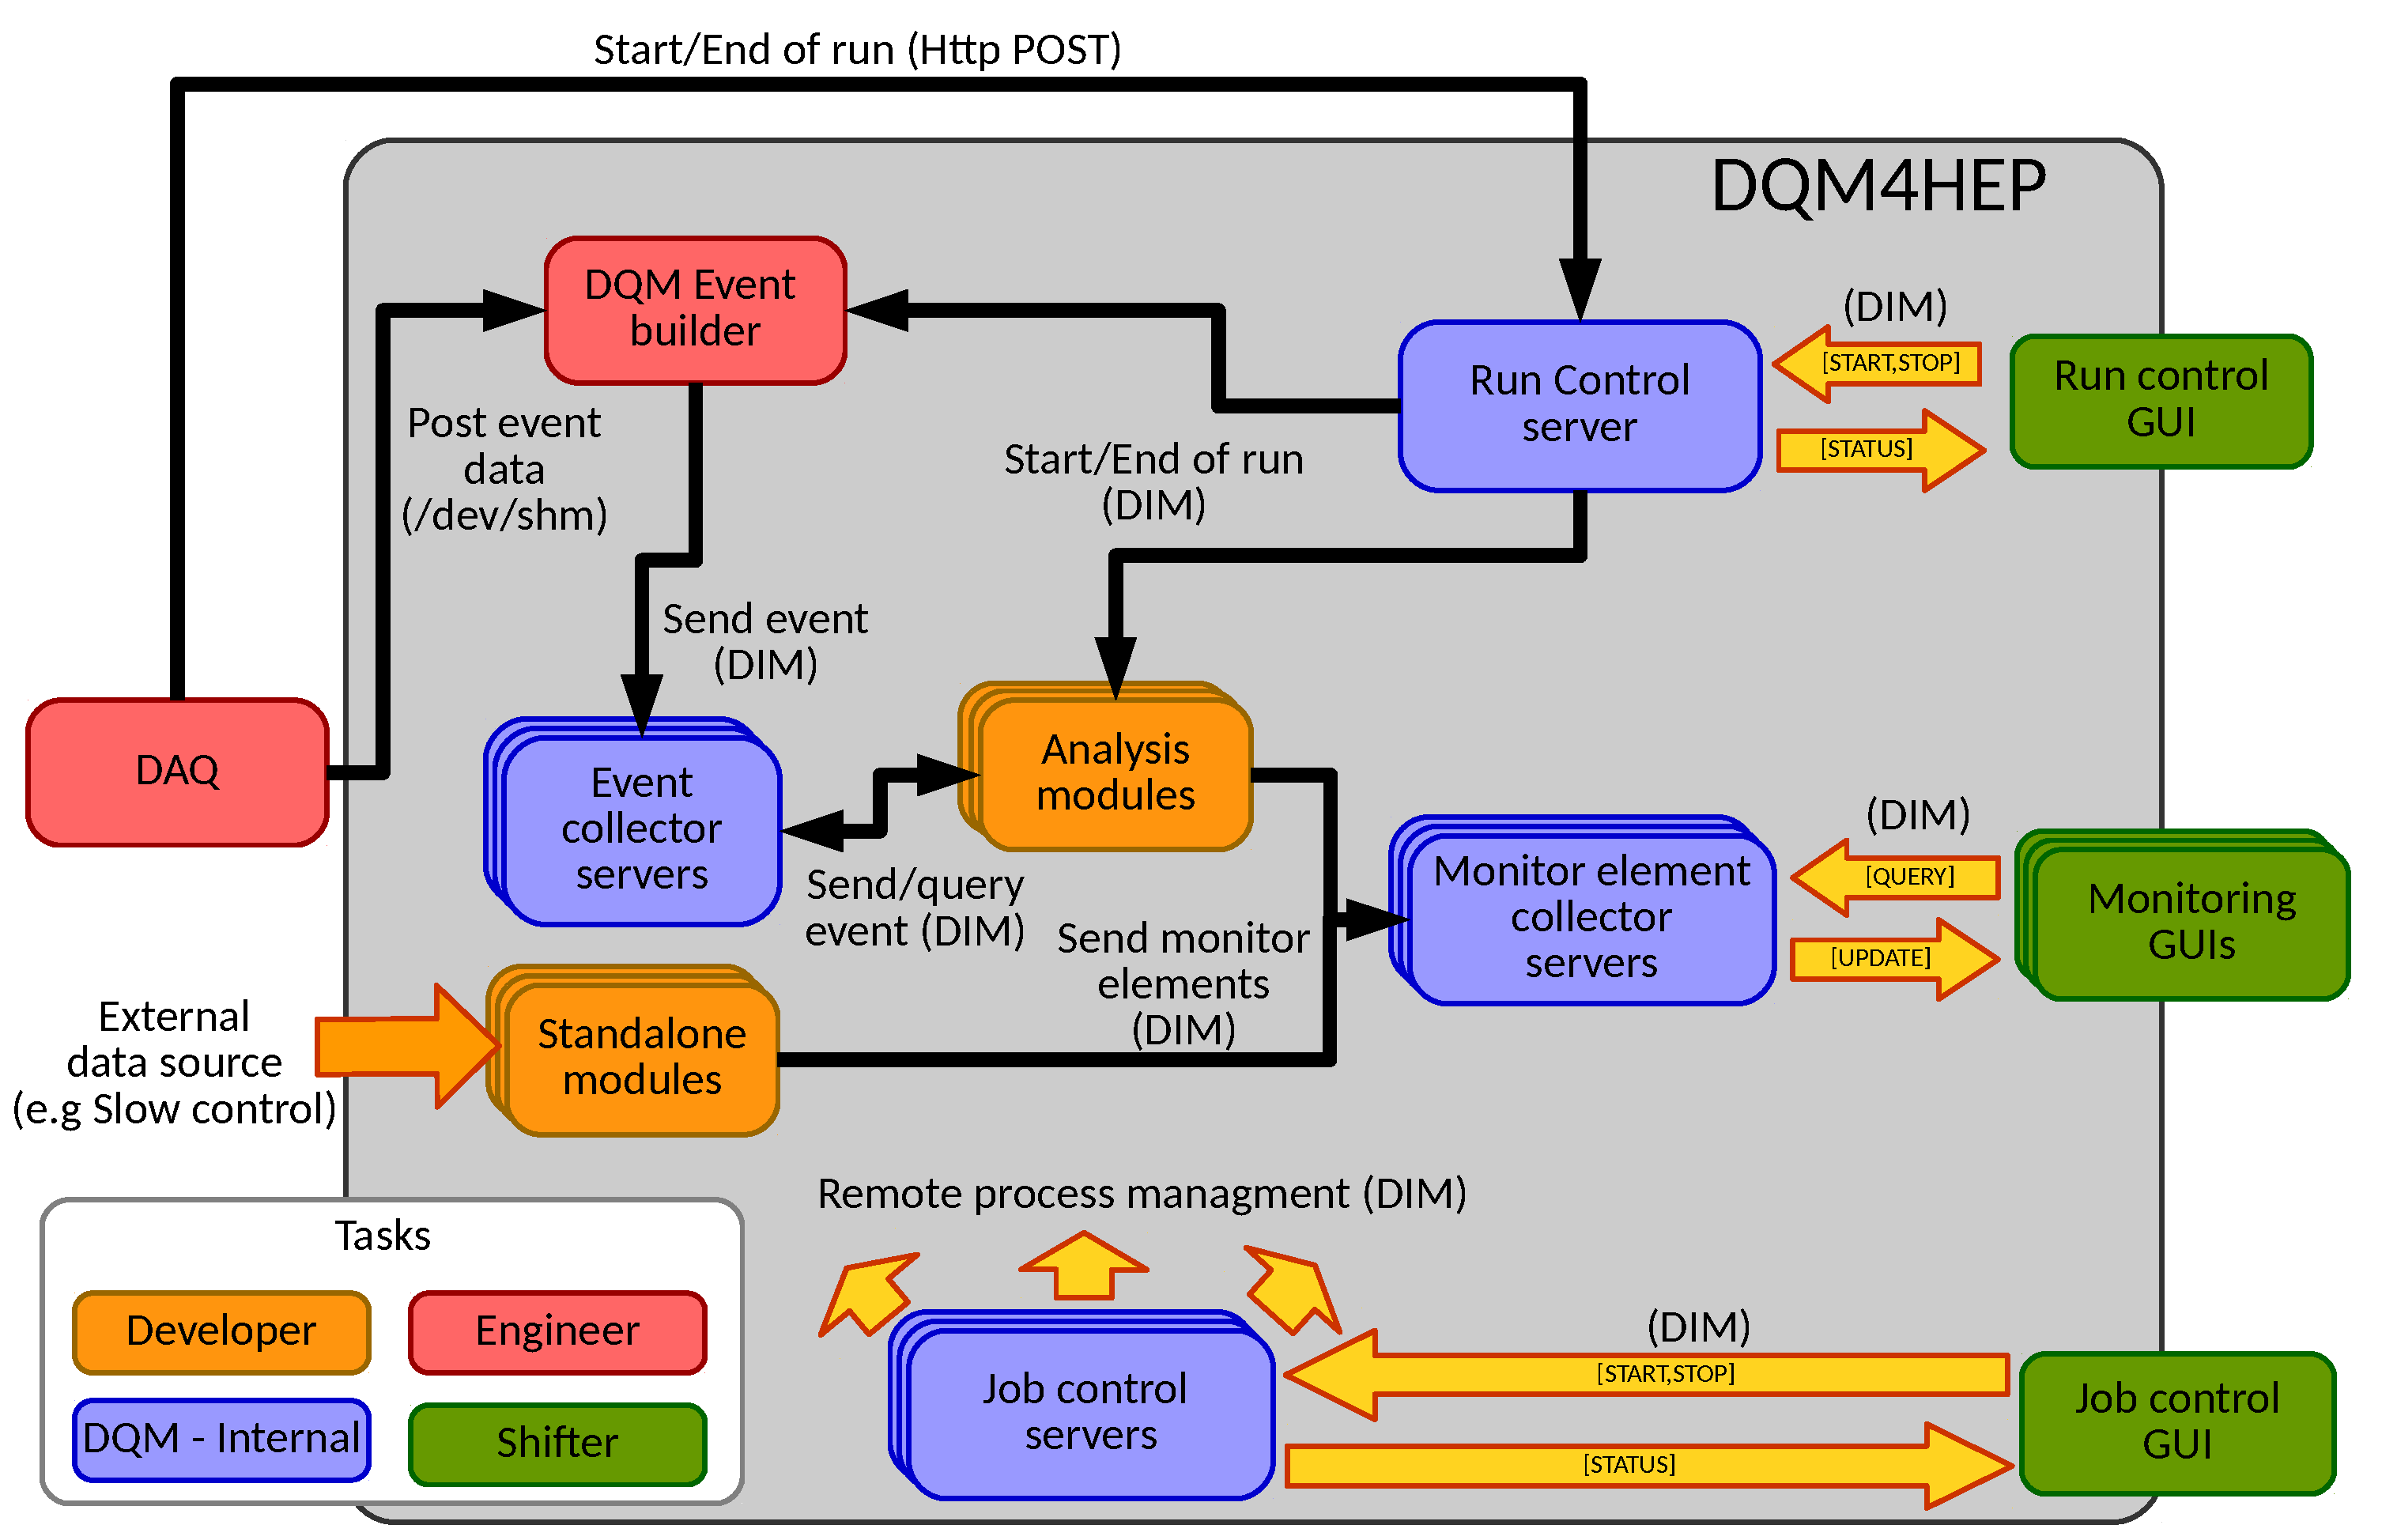
\includegraphics[width=0.95\textwidth]{../Pictures/GlobalArchitectureDiagram.pdf}
	\caption{The global online architecture of DQM4hep. Each block is colour-coded to show which operator of the testbeam is responsible for the process.}
	\label{figure:daq/dqm4hep/architecture}
\end{figure}

\begin{figure}[p]
	\centering
	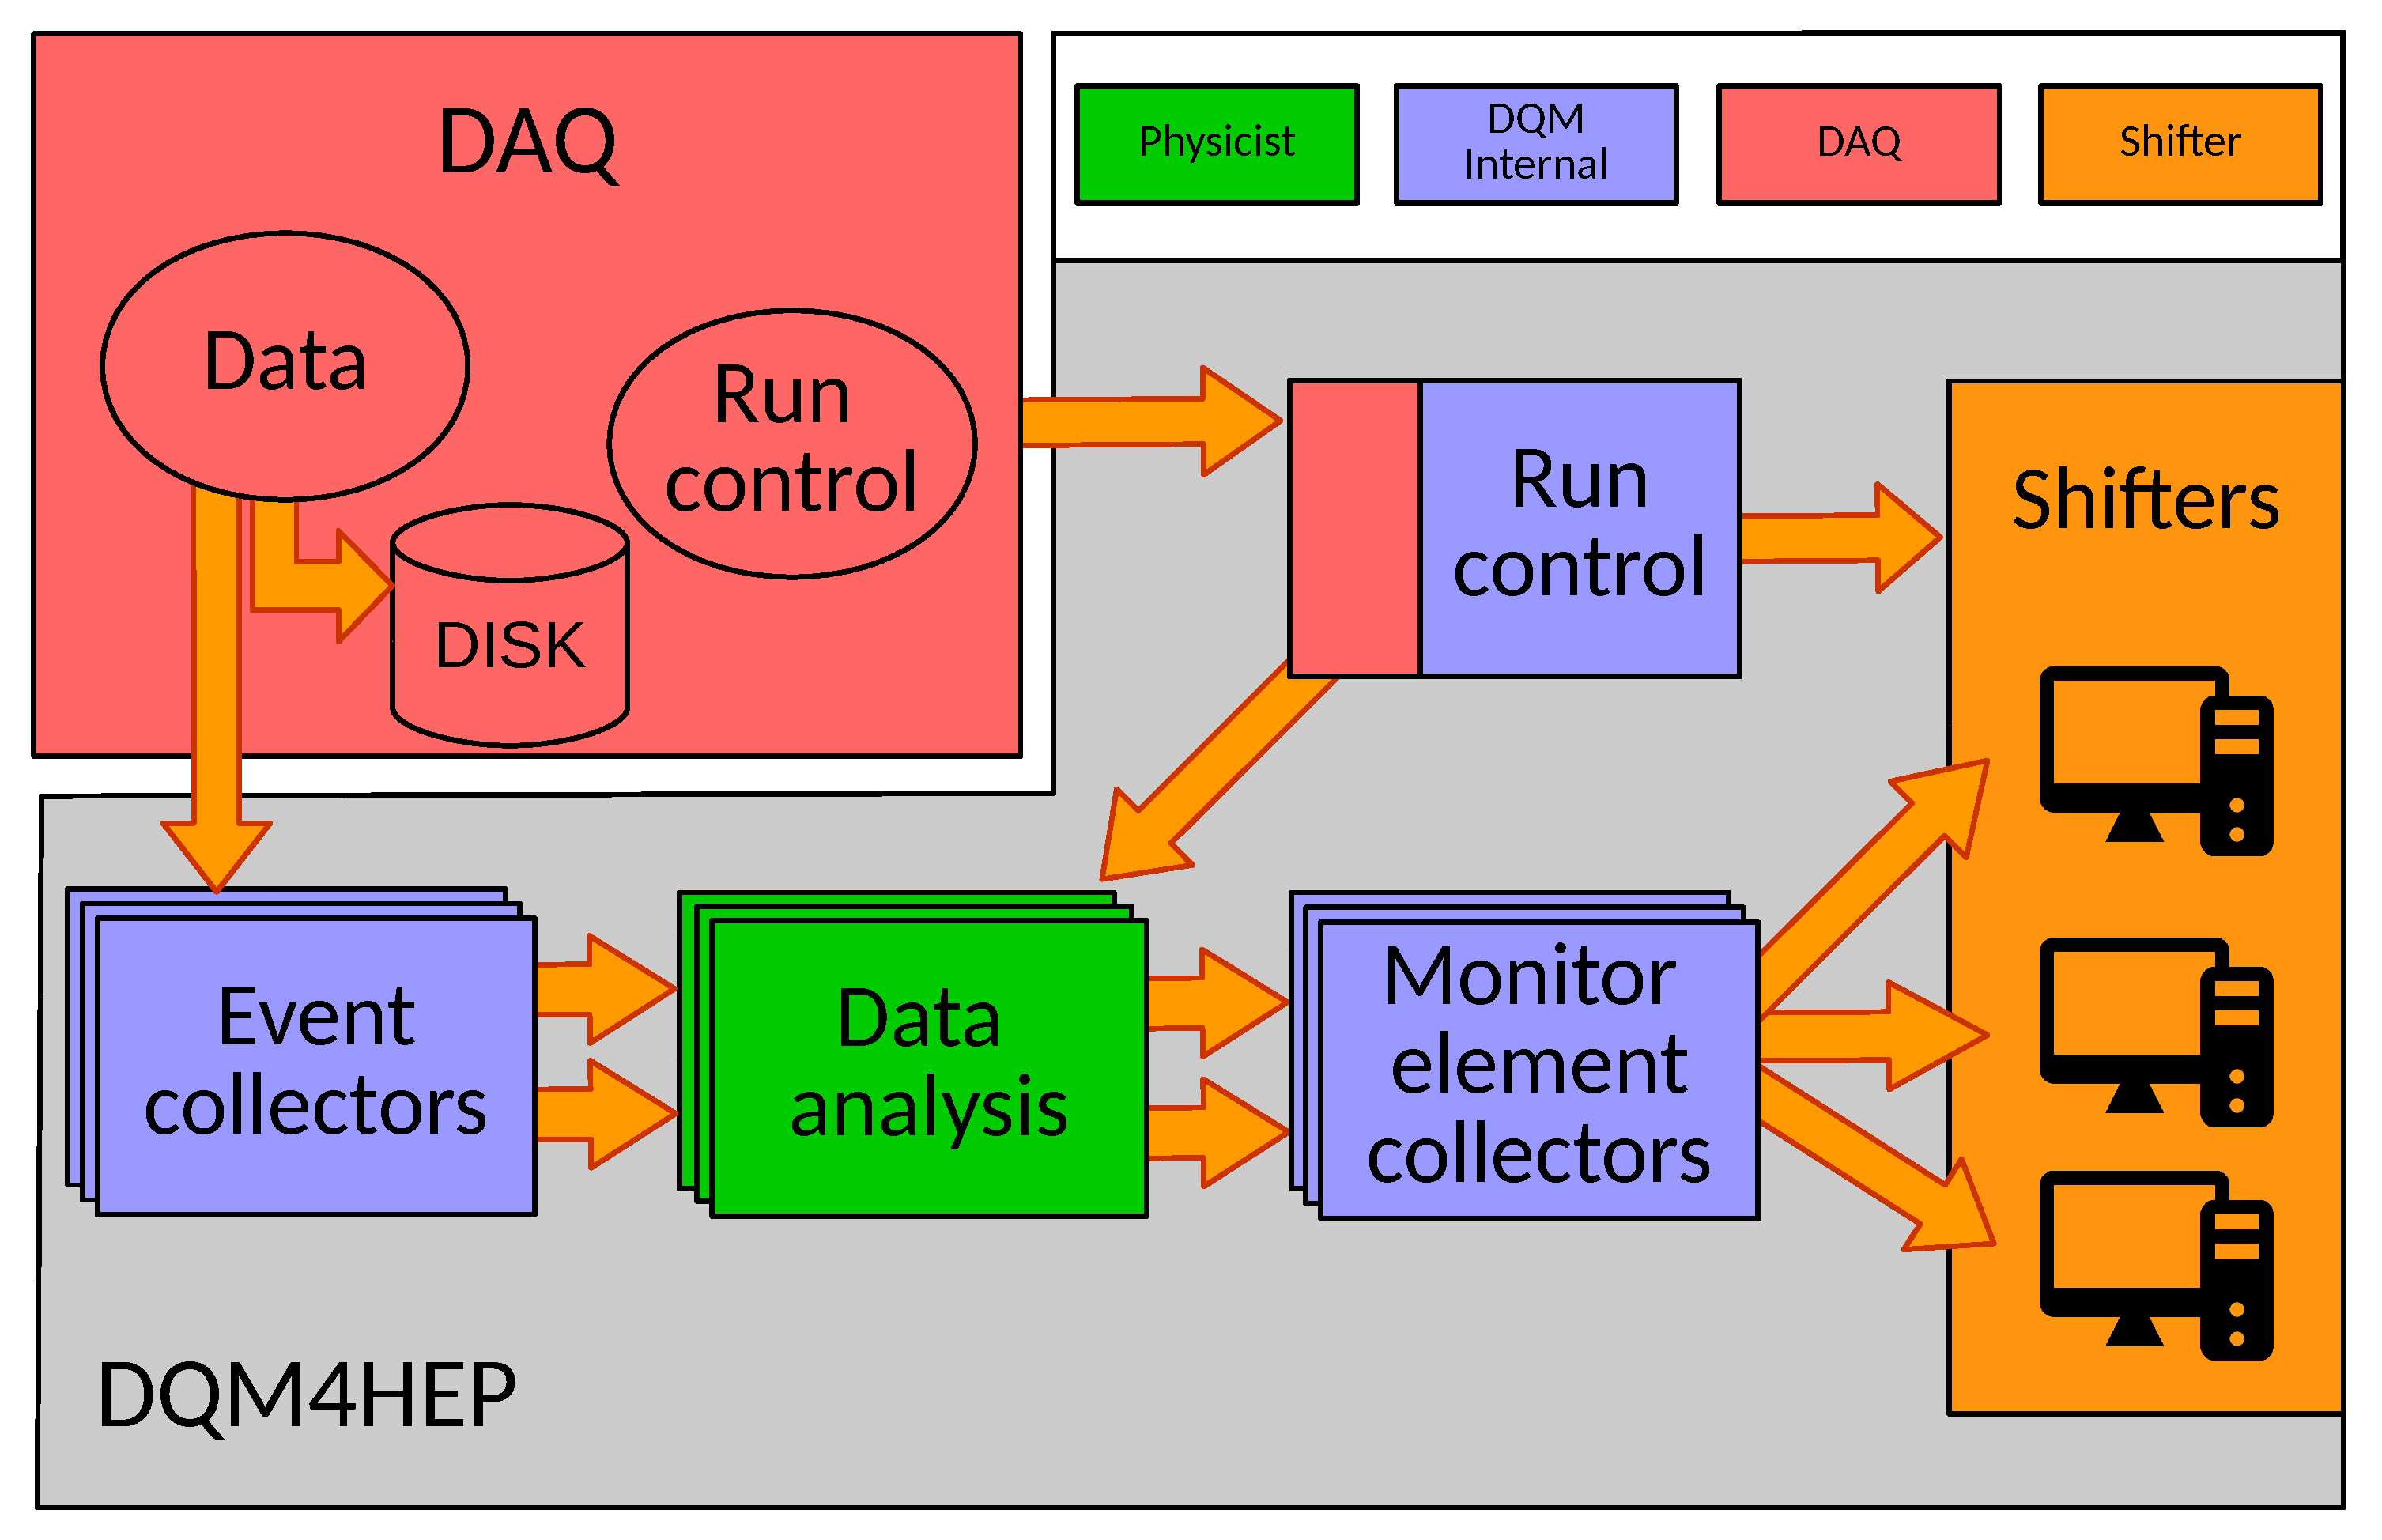
\includegraphics[width=0.95\textwidth]{../Pictures/AnalysisModuleArchitecture.pdf}
	\caption{The structure of running DQM4hep online using an analysis module.}
	\label{figure:daq/dqm4hep/analysis-module}
\end{figure}

\subsubsection{Analysis modules}
Analysis modules recieve events from the data aquisition system, processing the data according to a user-specified procedure to create ROOT TObjects like histograms, graphs, plots, etc. The analysis module then handles encapsulating these objects as monitor elements, and sending them to the rest of the framework for display and storage. 

An analysis module is specific to one use case, and is intended to be written by the user with their data format and processing needs in mind. However, the framework provides both templates and examples for how to write an analysis module. 

An example of the structure of the framework utilising an analysis module can be seen in Fig. \ref{figure:daq/dqm4hep/analysis-module}.

\subsubsection{Standalone modules}
Standalone modules are identical in form to analysis modules described above. The distinction is that a standalone module does not operate on data coming from the data aquisition device. One of the intended and most common usages of standalone modules is as a slow control, taking data from monitoring sensors on the device rather than data, to report on the condition of the hardware. Standalone modules could also be used to \emph{generate} data, if needed, acting as a programmed signal generator or random number generator. 

An example of the structure of the framework utilising a standalone module can be seen in Fig. \ref{figure:daq/dqm4hep/standalone-module}.

\subsubsection{File reader plugins}
A file reader is a type of plugin that reads a file from the disk and packs it into a data structure necessary for usage within DQM4hep. They are used primarily for offline monitoring or data processing. File readers can be made for any kind of file, provided the user understands the data structure. There are existing examples of file readers for data stored as binary, plain text, LCIO files, and ROOT TTrees. 

An example of the structure of the framework utilising a file reader plugin can be seen in Fig. \ref{figure:daq/dqm4hep/file-reader}.

\begin{figure}[p]
	\centering
	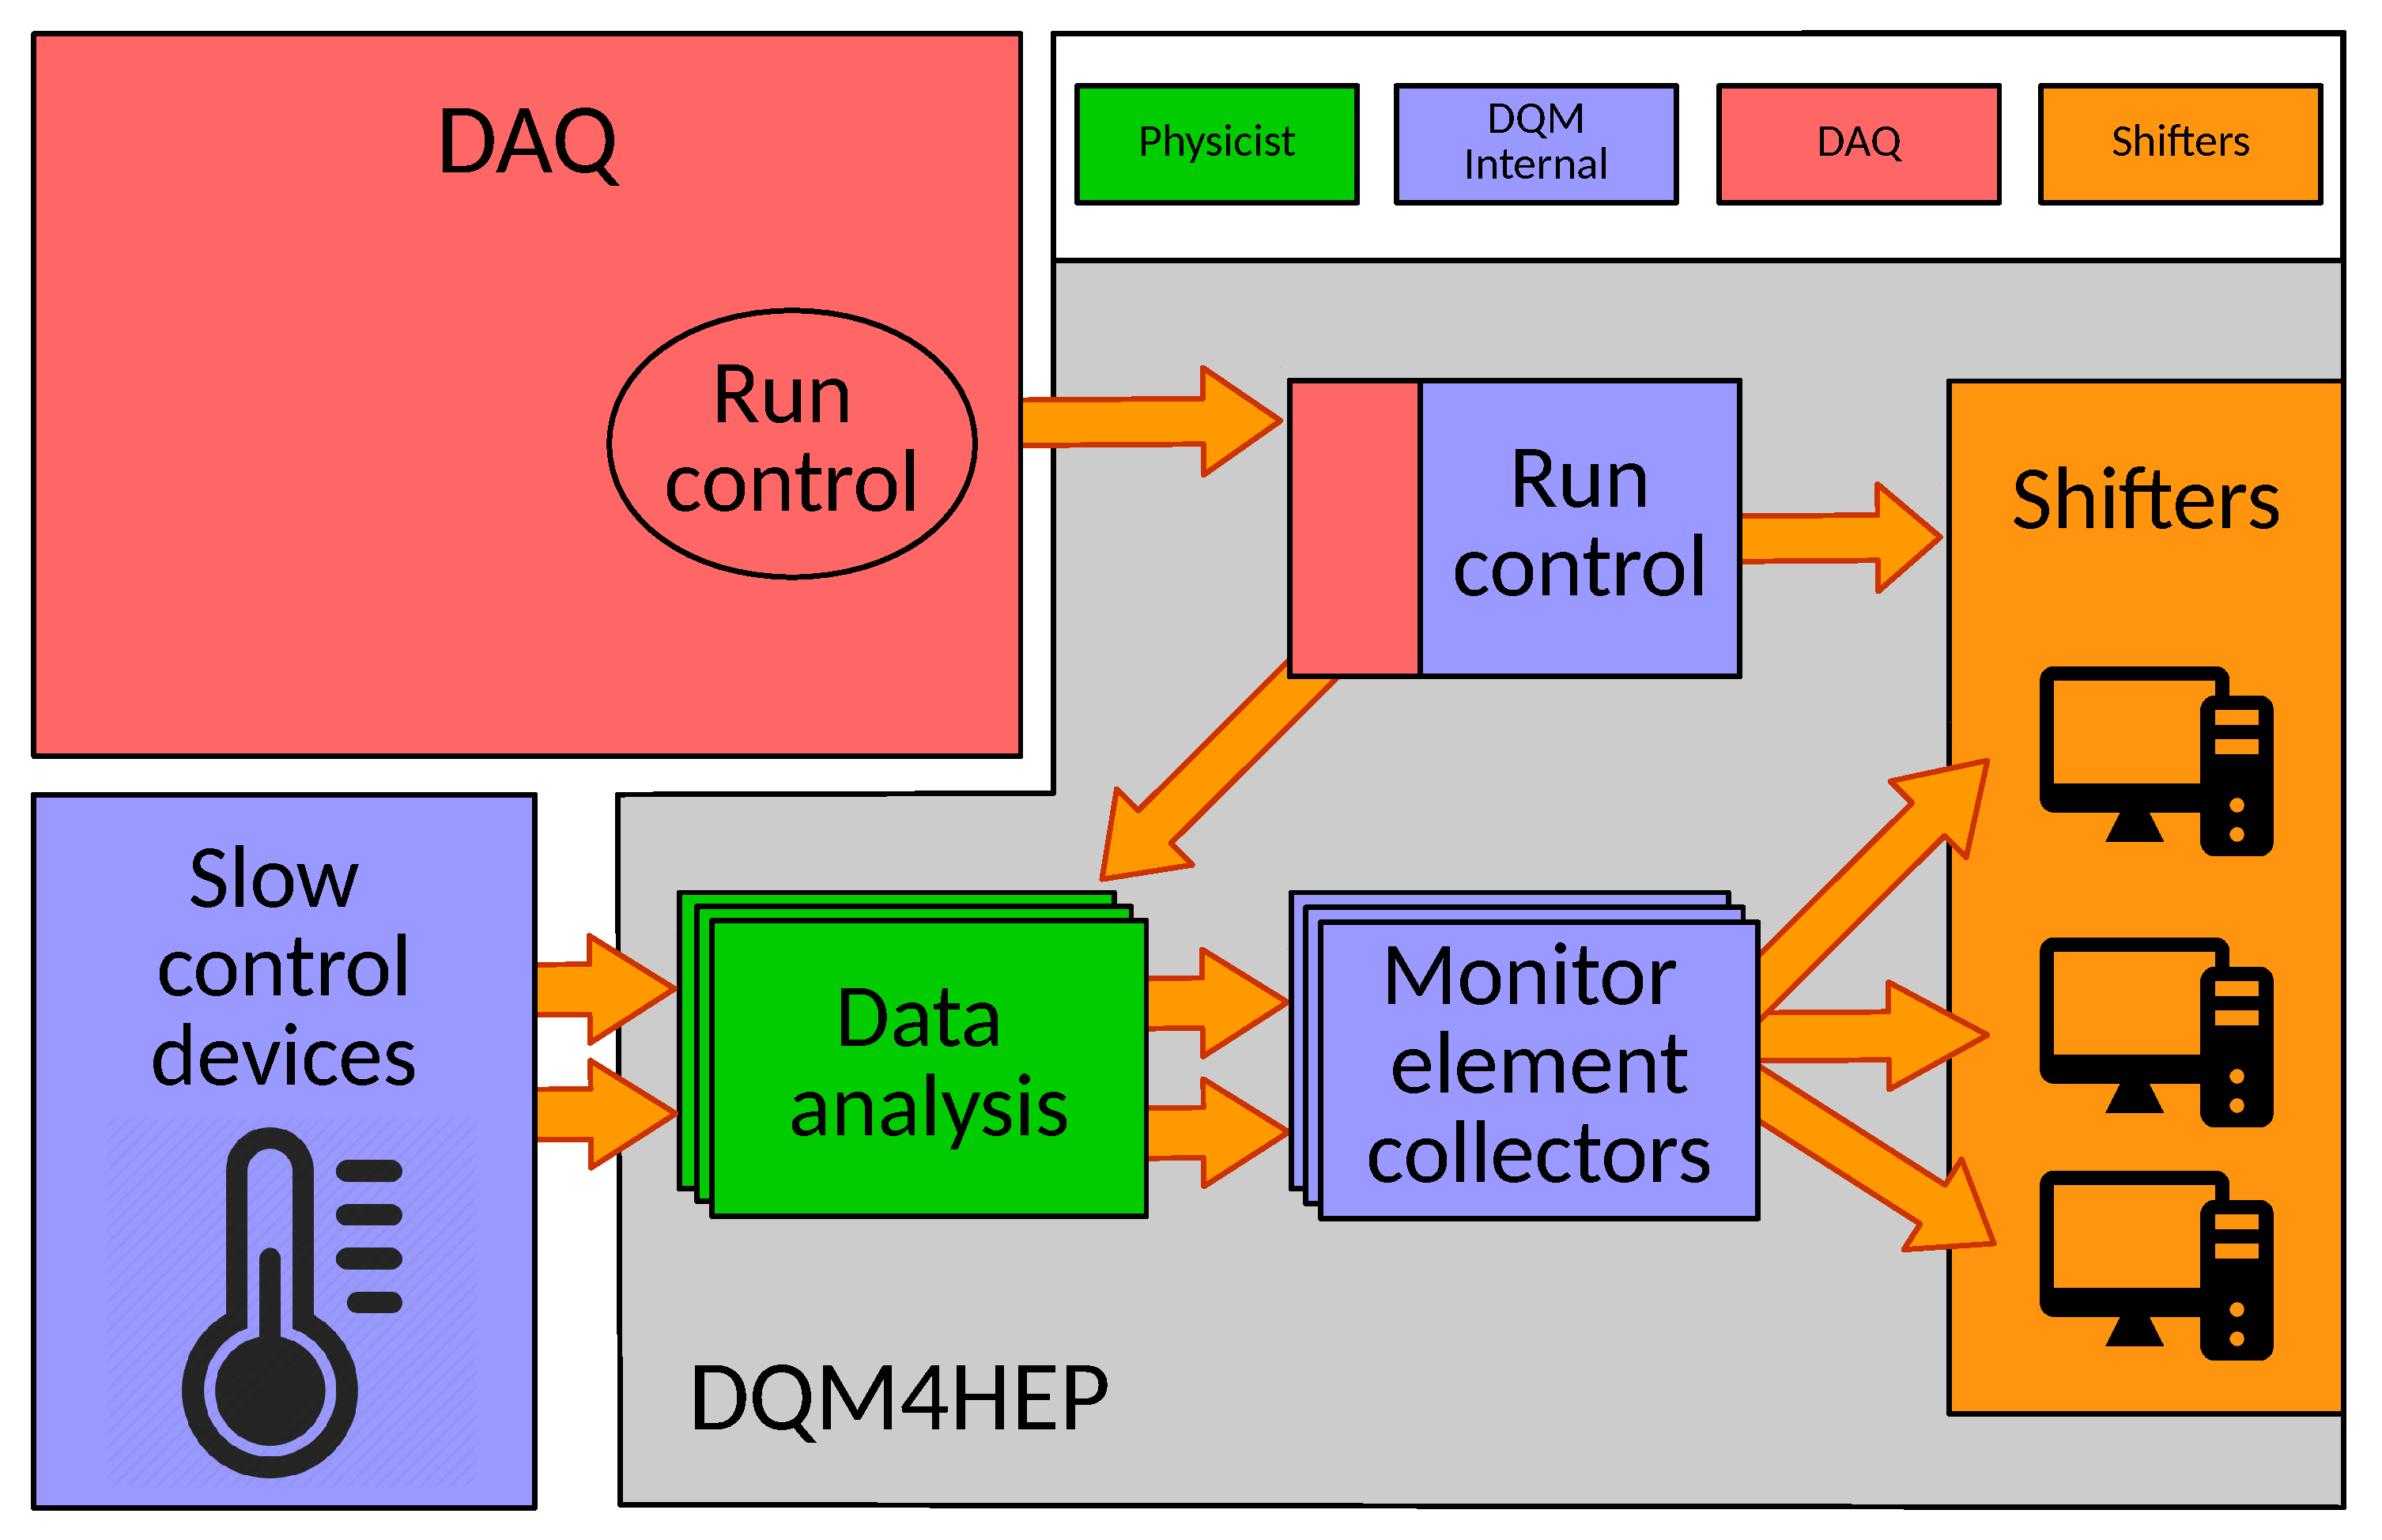
\includegraphics[width=0.95\textwidth]{../Pictures/StandaloneModuleArchitecture.pdf}
	\caption{The structure of running DQM4hep online using a stand alone module.}
	\label{figure:daq/dqm4hep/standalone-module}
\end{figure}

\begin{figure}[p]
	\centering
	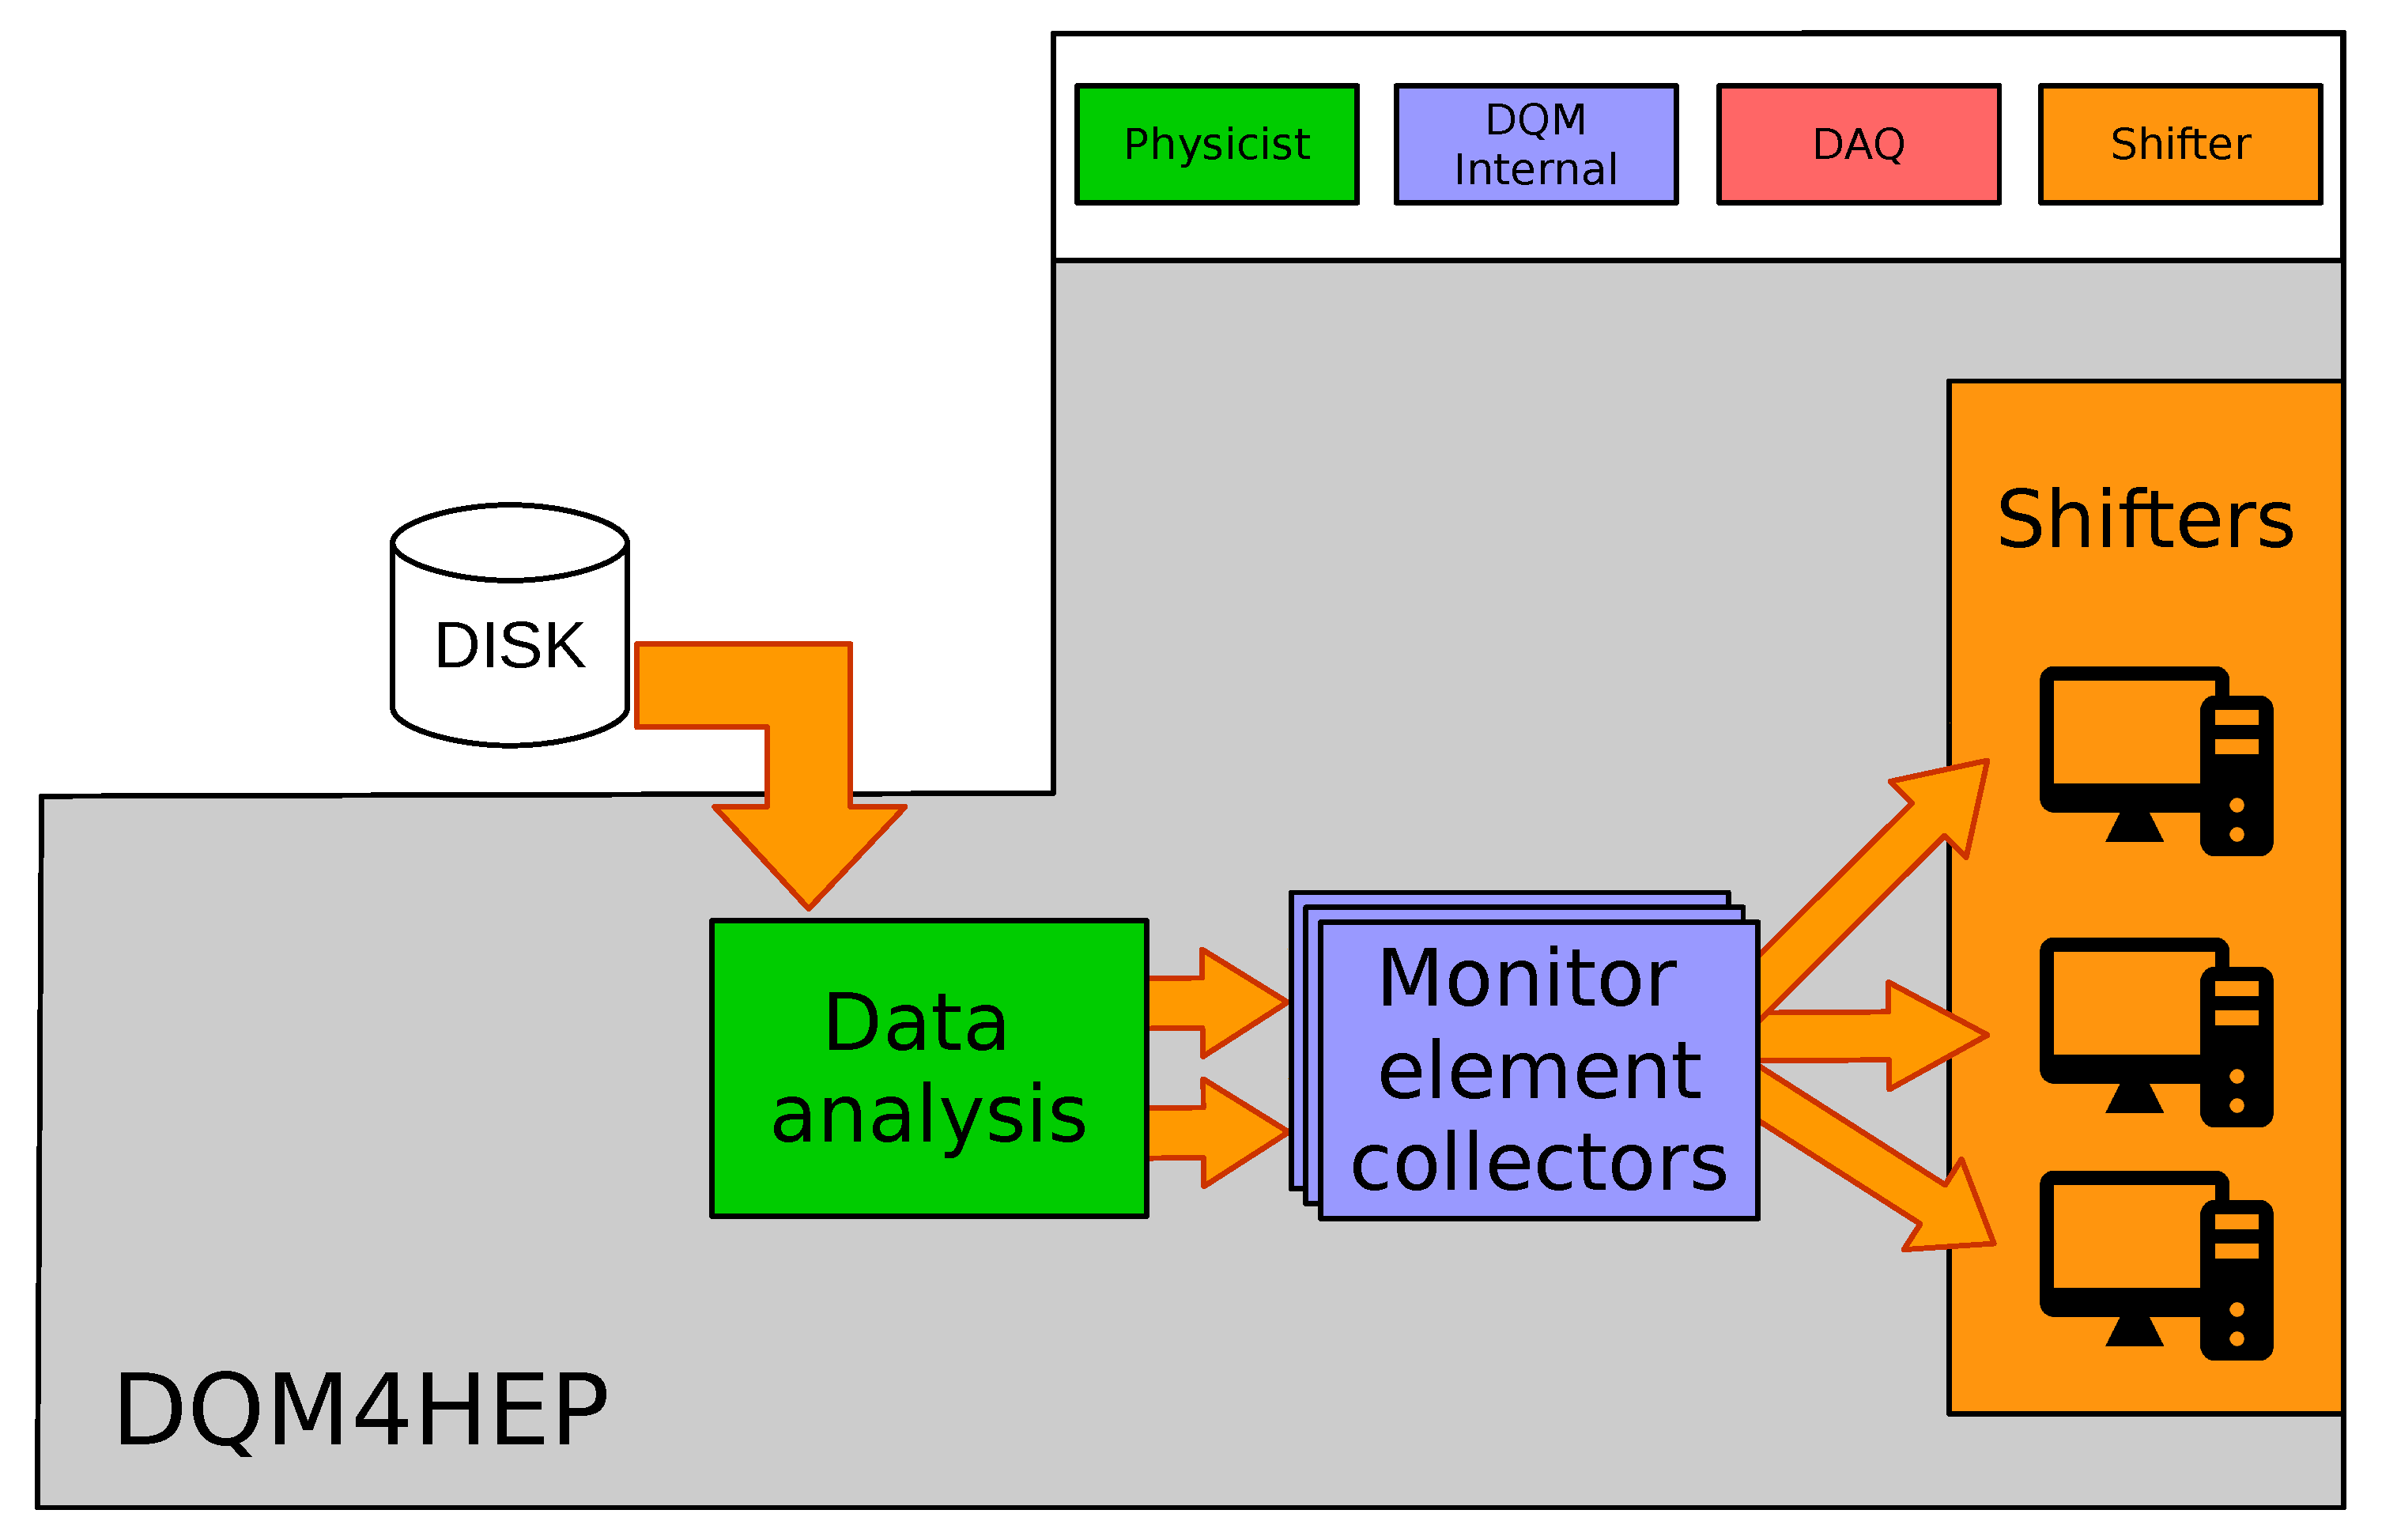
\includegraphics[width=0.95\textwidth]{../Pictures/FileReaderModuleArchitecture.pdf}
	\caption{The structure of running DQM4hep offline using a file reader module.}
	\label{figure:daq/dqm4hep/file-reader}
\end{figure}

\subsubsection{File streamer plugins}
A file streamer is a type of plugin that reads data from a stream and packs it into a data structure necessary for usage within DQM4hep. They are for receiving data from a data acquisition device for online monitoring. File streamers can be made for any kind of data stream, provided the user understands the data structure. File streamers are considered the ``default'' in DQM4hep.

\subsection{Visualisation and graphical user interface}
As of writing, the graphic user interface (\acrshort{GUI}) and visualisation elements of the framework are still under active development for a new version. Therefore this topic will be split into two sections: one to describe the existing GUI, and one to discuss the motivations and goals for the new GUI under development. 

\subsubsection{Current GUI and visualisation} 
The current version of the GUI is built with Qt, a free and open-source toolkit and framework for creating OS-independent graphic user interfaces and widgets. The motivation for choosing Qt was that ROOT provides an option for integration between ROOT and Qt, allowing ROOT classes like \texttt{TCanvas} to be ``embedded'' into Qt widgets. This simplified the implementation of a GUI, allowing a graphical interface based on Qt to be written, then graphics from ROOT simply opened within the existing widgets and windows. % We should cite this; this information is from here: (https://root.cern.ch/root/html534/guides/users-guide/ROOTandQt.html). 

This interface is used in multiple places, including the run control process and the monitoring GUI. The monitoring GUI is built on a system of canvases. Each canvas can have multiple plots open, which can be resized, maximised, minimised, etc. and manipulated as normal for ROOT plots. The user can also create new canvases for more space to arrange plots.

In addition to this, there is an optional provision for a monitoring steering file, which contains presets of canvases, and the plots displayed on them. This is extremely useful when dealing with large datasets or large numbers of plots, as the plots required by the user can be opened automatically when the monitoring interface is run.

An example of the Qt-based monitoring GUI in use can 3be seen in Fig. \ref{figure:daq/dqm4hep/old-gui}. 

\begin{figure}[h]
	\centering
	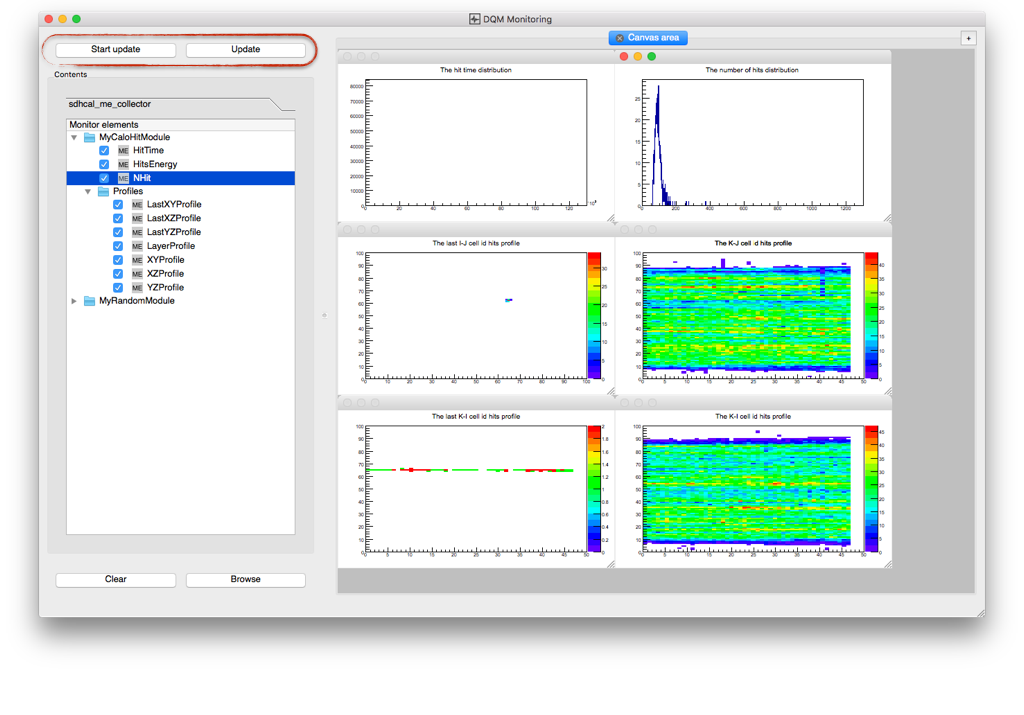
\includegraphics[width=1.0\textwidth]{../Pictures/DQM4hepMonitoringGui.png}
	\caption{An example of the current Qt-based monitoring GUI in use.}
	\label{figure:daq/dqm4hep/old-gui}
\end{figure}

\subsubsection{New user interface and visualisation package}
For the newer versions of DQM4hep, the decision was made to overhaul the GUI and visualisation packages, removing Qt from the framework and moving to a web-based interface.

The removal of Qt was motivated by two reasons. Firstly, the integration with ROOT provided some complications, since running DQM4hep's Qt-based GUI requires an installation of ROOT compiled with the \texttt{--enable-Qt} flag enabled. The majority of ROOT installations in remotely-accesible file systems based at CERN and DESY (which are heavily used for analysis and testbeams) were not compiled this way. Secondly, Qt was an additional dependency that must be installed prior to use, making the software more dependent upon the operating system, compiler tools, and environment of the machine, and thus less generic and easy to use. % Also isn't Qt support getting removed from ROOT soon? We'd need a citation for that though.

The removal of the Qt UI allows for greater freedom with UI development. The intended goal is to have a browser-based GUI, removing dependency on any external GUI libraries and allowing it to function on any device. This will also make it more user-friendly and convenient, as the interfaces for run control, networking, and data monitoring and quality display can be simply run in different tabs of a web browser.

As of writing, the web interface is under active development by R\'{e}mi Et\'{e} and is not yet complete. However, a mock-up of the web interface can be seen in Fig. \ref{figure:daq/dqm4hep/future-gui}.

\begin{figure}[h]
	\centering
	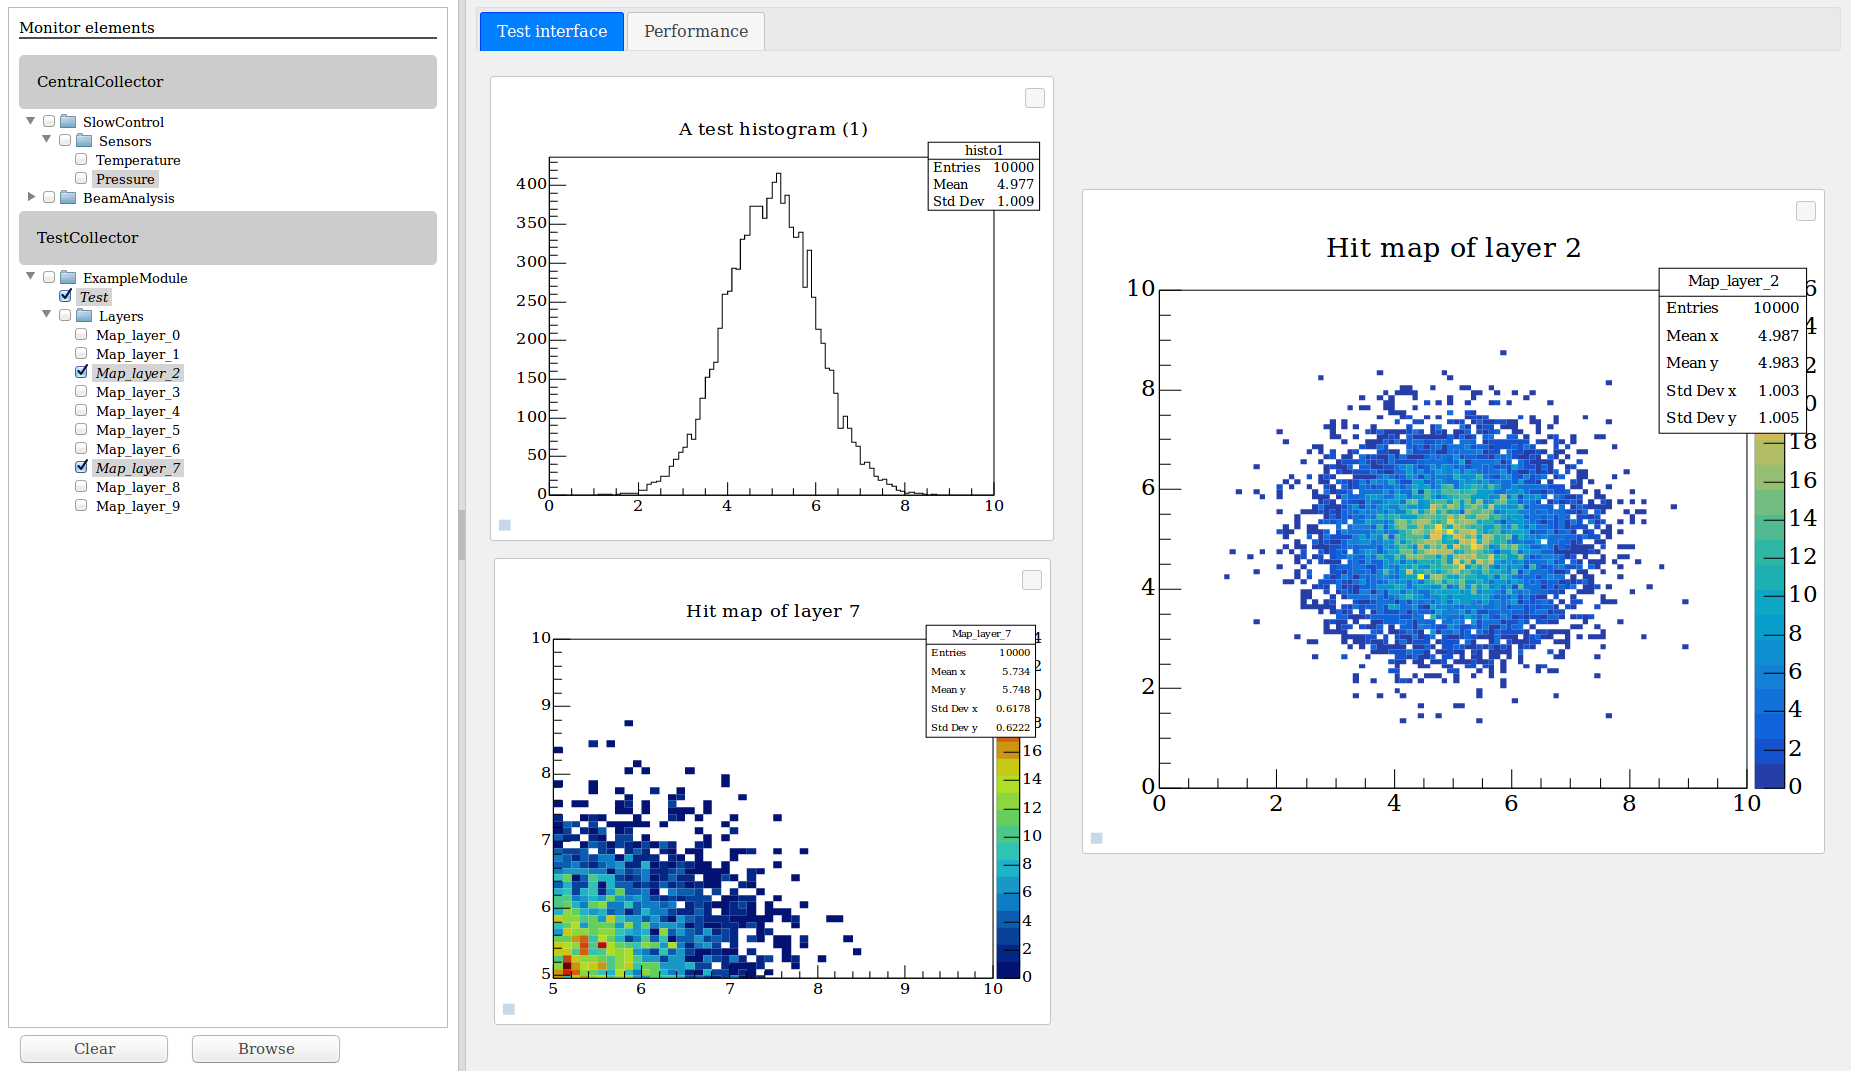
\includegraphics[width=1.0\textwidth]{../Pictures/ScreenshotWebMonitoring.png}
	\caption{A preview of the planned web-based monitoring interface.}
	\label{figure:daq/dqm4hep/future-gui}
\end{figure}

\section{Data quality monitoring} % Maybe examples of qtests in action?
Data quality monitoring is a type of data monitoring where the data is tested using some form of statistical or mathematical process to produce a value corresponding to the ``quality'' of the dataset. This can take many forms, such as comparing an experimental dataset to reference data acquired from previous experiments, or requiring that the $\chi^2$ or p-value of a dataset may need to pass a certain threshold to be considered valid.

The definition of the ``quality'' statistic will differ according to a variety of factors such as the type of data, the aim of an experiment, etc. Common examples are p-values, or binary tests where data that passes had a quality of 1, and 0 otherwise.

One of the benefits of data quality monitoring is that it provides a more reproducible and robust set of checks on data-taking, allowing quantitative analysis of the performance of a detector prototype. It can also be used as a way for shifters without detailed knowledge of the hardware, software, or physics to determine whether the detector is performing as intended during a testbeam when experts are not available, by using the quality statistics as a guide.

Previous versions of DQM4hep did not have infrastructure to support data quality monitoring, but this was added during refactoring in preparation for the next release version. Once this was in place, this permitted an array of quality tests to be developed, implemented, and tested. 

A quality test (or `qtest') processes a series of monitor elements (ROOT TObjects) according to a set of criteria defined in the test's code. This test produces a numberical result between 0 and 1, referred to as the ``quality''. Within the framework, quality tests are self-contained C++ code files, which hook into the framework's system for execution. Quality tests are run by using the executable \texttt{dqm4hep-run-qtests} and a steering file to define paramters, such as which files to load, which quality tests to execute, and what the passing and failing boundaries are for each quality test. 

The quality tests that have been implemented in DQM4hep are described in detail below. Each test requires a certain type of object as an input and has it's own definition of what the ``quality'' statistic represents. Some quality tests also require a reference to compare against the input data, which is also described.

\subsection{Property within expected test}
This is a quality test that takes either a TH1 or TGraph object, and finds some user-defined parameter. The parameter must be one of: mean, mean90, root mean square (RMS), root mean square 90 (RMS90), or median. It then checks whether either: that this parameter is within a user-specified range; or that it is above or below the user-specified threshold. If a range is being used, the result is the p-value of the property being within the specified range. If a threshold is being used, then the result is 1 if the property passes the threshold, 0 otherwise.

\subsection{Exact reference comparison test}
This is a quality test that takes any TObject, and compares it to a user-specified reference object (which must be of the same type). The result is 1 if the two objects are exactly identical, 0 otherwise. 

\subsection{Fit parameter in range test}
This is a quality test that takes either a TH1, TGraph, or TGraph2D object and plots a user-defined function onto it, solving for one of the parameters of the function, then checks it against a user-defined range. The result is the p-value of the parameter being within the specified range.

\subsection{Kolmogorov-Smirnov test}
This is a quality test that takes either a TH1 or a TGraph object, and performs the Kolmogorov-Smirnov test between that object and a specified reference. The result is the p-value of the Kolmogorov-Smirnov test. The Kolmogorov-Smirnov test is intended for unbinned data, not histograms, but ROOT provides a function for performing the Kolmogorov-Smirnov test on histograms, so this is functionality is also included for the sake of completeness.

\subsection{Pearson $\chi^2$ test} % We should probably cite the Pearson chi^2 test itself
This is a quality test that takes a TH1 object and performs the Pearson $\chi^2$ test between that object and a specified reference. This test is analogous to the Kolmogorov-Smirnov test, but is designed specifically to work for binned histogram data. The result is the p-value output by the $\chi^2$ test. 

\section{Adaptation to other detectors}
Due to the modularity and genericity of DQM4hep, the process of deploying it for a new detector is simple -- the only parts of DQM4hep that need to be made for any specific use case are the analysis modules, standalone modules, streamer plugin, and file reader plugin. For all of these plugins, there are templates available in the codebase, as well as examples of in-use plugins for other detectors. A few special DQM4hep-specific functions are necessary for these plugins to hook into the framework properly, but apart from these all user-provided plugins are written in normal C++ code that also integrates ROOT, so should be familiar to most users.

A file streamer or file reader must be written by the user given a specific data structure. This requires knowledge of both the event data model of the data acquisition setup, as well as the structure of the data files. The ideal person to write this code is someone with detailed knowledge of the data acquisition software being used, and the data storage or streaming. 

In general, only one of the file streamer or file reader plugins will be needed. Both of these plugins are similar in structure and differ only on where they get the data from -- a file reader loads a file from disk, whereas a streamer loads it from the data acquisition system. If the data will be monitored offline or ``nearly-online'' by loading files from disk, then a file reader plugin must be written. If the data is to be monitored online, then a streamer plugin must be written. 

Once the information is accessible from either the file reader or streamer, the framework handles passing this data to the analysis modules. Analysis modules are a type of plugin which take data that has been packaged into events by a file reader or streamer plugin and performs some analysis on it. The main action an analysis module must do is create a monitor element (a ROOT TObject) then emit it to the rest of the framework. Before this step an arbitrary amount of processing can be done, e.g. checking validation bits, thresholds, error-checking, and so on. Monitoring the data quality can be done from within analysis modules but this is not recommended as dedicated quality tests (see section above) are available.

For each analysis module that is being run, an XML steering file is required to provide the parameters and networking information to all the processes needed. A single steering file can call only a single analysis or standalone module, but multiple steering files can be run in parallel by the framework.

Examples of using DQM4hep with testbeams both within the AIDA-2020 community and outside of it can be found in Chapters \ref{chapter:aidatestbeams} and \ref{chapter:ideatestbeam}, respectively.

\section{Documentation and user manual} 
One of the biggest hurdles for the promotion and uptake of a new framework is the lack of understanding or familiarity with it's use. Many research teams will continue to use existing software solutions, which may be suboptimal or difficult to use, according to the principle of ``better the devil you know than the devil you don't''. The first step to overcoming this is to produce clear, readable and complete documentation across the entire range of features the framework has.

The DQM4hep framework has two sets of documentation with different intended readers and different aims, so these will be discussed separately.

\subsection{Doxygen documentation}
Doxygen is a tool for automatically generating documentation resources for C++ code, relying on marked secctions of documentation written within the actual code itself. Doxygen is able to directly obtain the sturcture of code, objects, functions, etc. from the code, allowing it to automatically generate a complex and rich set of documentation that categorises and indexes objects based on their inheritance, namespace, etc.

Doxygen can also generate an HTML- or \LaTeX -based document that can be used as a local reference guide or hosted online. This makes Doxygen a powerful tool for documenting the technical aspects of code, demonstrating hierarchies of functions and objects, and an extremely useful reference guide for large programs or frameworks.

While Doxygen documentation is extremely useful, it does have some limitations. Doxygen functions more as a technical reference for code, lacking any overviews or instructions due to it's automatic generation. This kind of documentation lacks a holistic element, and has no way for new users or those less familiar with the codebase to understand the overarching concepts. This can make it inaccessible for new users. The way this was addressed will be dicussed in the next section.

DQM4hep has a Doxygen website hosted on the internet, which is available here\cite{dqm4hep-doxygen}.

\subsection{User manual} % include elements of the documentation and overview of how to use program as a whole; examples of use.
The existing documentation featured the common elements of the framework -- such as the plugin system, event interface, logger, and XML parser -- explained in detail, with clear examples and straightforward advice on their use.

My contribution to this was to write in-depth explanations on the structure, usage, and creation of analysis modules and quality tests, the two parts that are most specific to end-users. The experience I acquired using the framework and deploying it on testbeams for the first time, as well as integrating it with different detectors, provided a strong knowledge base to write the user manual intended for a user approaching the framework for the first time. These testbeams are described in more detail in Chapters \ref{chapter:aidatestbeams} and \ref{chapter:ideatestbeam}.

The user manual can be found online here\cite{dqm4hep-user-manual}.

\subsubsection*{Analysis module guide}
There is an in-depth explanation of each of the component functions of an analysis module, discussing which actions or data processing should be done in each, and their intended purposes. There is also an explanation of the XML steering files that are necessary to run an analysis module, and instructions on how the executable is run, along with it's arguments.

In addition to this there is a worked example of an analysis module from start to finish. A simplified particle physics detector and it's data format is defined, and then the reader is lead through the process of writing an analysis module step-by-step and function-by-function to obtain certain plots and results from the data. This is intended to give a more concrete demonstration of usage, as an easier to follow example. This section is also written in simple and plain English in order to be as accessible as possible.

Along with this documentation there is the \texttt{dqm4hep-example} Github repository [cite], which contains all of the code used in the analysis module user manuals, as well as the required cmake and make files to begin compiling projects right away. The intention of this repository is for new users to make a copy, write their own modules, and have everything needed for compiling and running them ``out of the box'' straight away. The user manual references this repository, so that users can see the files from the worked example in their full form.

\subsubsection*{Quality testing guide}
There is extensive documentation of quality testing; each quality test is described in detail, including their purpose, output, required parameters, and optional parameters. In addition to this, there is a guide for how to run quality tests, including an explanation of running from the command line and an in-depth look at the structure of the XML steering files required.

Finally there is a section explaining how to write new quality tests. This includes a detailed explanation of the purpose of each function within a quality test file, what the required outputs are and how to utilise them, error testing, and advice on maintaining a style consistent with the rest of the framework.

%\textbf{Running a quality test}
%
%Quality tests can be run using the \texttt{dqm4hep-run-qtests} executable, found in \texttt{dqm4hep-core/bin/}. This executable handles the running of the actual binaries for each qtest, as well as obtaining monitor elements from the ROOT file and the setting of parameters. This executable has one required arguments and several optional ones, detailed below. 
%
%\textbf{Arguments}
%
%\begin{verbatim}
%-h
%--help
%\end{verbatim}
%
%Displays usage information, then exits.
%
%\begin{verbatim}
%-i <string>
%--input-qtest-file <string>
%\end{verbatim}
%
%(Required) Gives the path to the XML steering file that defines what quality tests to run, their parameters, and what monitor elements to run them on. See the section below for more information on these steering files.
%
%\begin{verbatim}
%-c
%--compress-json
%\end{verbatim}
%
%Turns on compression for the JSON qtest report output file. Off by default.
%
%\begin{verbatim}
%-w
%--write-monitor-elements
%\end{verbatim}
%
%Turns on writing of monitor elements in the qtest report. Off by default.
%
%\begin{verbatim}
%-p <string>
%--print-only <string>
%\end{verbatim}
%
%%Prints only the quality reports of the given flag. Options are \texttt{undefined}, \texttt{invalid}, \texttt{insuf_stat}, \texttt{success}, \texttt{warning}, \texttt{error}.
%
%\begin{verbatim}
%-e <string>
%--exit-on <string>
%\end{verbatim}
%
%Forces the program to exit if any qtest results in the given code. or greater. Options are \texttt{ignore}, \texttt{failure}, \texttt{warning}, \texttt{error}. This is \texttt{failure} by default.
%
%\begin{verbatim}
%-v <string>
%--verbosity <string>
%\end{verbatim}
%
%The verbosity of the logger. Options are \texttt{trace}, \texttt{debug}, \texttt{info}, \texttt{warning}, \texttt{error}, \texttt{critical}, and \texttt{off}. This is \texttt{warning} by default.
%
%\begin{verbatim}
%-q <string>
%--qreport-file <string>
%\end{verbatim}
%
%Gives the path of the qtest report output file (in JSON) format.
%
%\begin{verbatim}
%-o <string>
%--root-output <string>
%\end{verbatim}
%
%Gives the path of a ROOT output file to save the processed mmonitor elements.
%
%\begin{verbatim}
%--
%--ignore_rest
%\end{verbatim}
%
%Ignores any arguments following this flag.
%
%\begin{verbatim}
%--version
%\end{verbatim}
%
%Displays version information, then exits.
%
%\textbf{Steering files}
%
%Steering files use XML to store all teh information needed to execute a qtest. An example steering file can be found in \texttt{dqm4hep-core/tests/test\_samples.xml}.
%
%There are two main sections: the \texttt{<qtests>} block and the \texttt{<monitorElements>} block, both of which must be within the \texttt{<dqm4hep>} XML tag.
%
%The \texttt{<qtests>} block defines the qtests to execute along with their settings or parameters, without reference to what they will be run on. The structure and parameters of these is highly dependent upon the qtest being used – see the section for each qtest above.
%
%The \texttt{<monitorElements>} block opens a file using the \texttt{<file>} tag, within which each monitor element is opened with \texttt{<fileElement>}. Inside this tag, all of the qtests to execute on this monitor element are given. In this example below, the qtests \texttt{ExampleTest1} and \texttt{ExampleTest2} are both performed on the monitor element \texttt{TestHistogram}:
%
%\begin{verbatim}
%<monitorElements>
%
%  <file name="test_samples.root">
%    <fileElement path="\TestDirectory" name="TestHistogram">
%    <qtest name="ExampleTest1" />
%    <qtest name="ExampleTest2" />
%    </fileElement>
%  </file>
%
%</monitorElements>
%\end{verbatim}
%
%Some kinds of qtests require reference objects to compare against, which must be declared in the \texttt{<references>} block. References have a \texttt{name} parameter which gives the path to the file used as a reference, and an \texttt{id} which is a short tag for referring to them later in the XML file. For example:
%
%\begin{verbatim}
%<references>
%  <file id="mc-ref" name="montecarlo_reference_samples.root"/>
%  <file id="ex-ref" name="experiment_reference_samples.root"/>
%</references>
%\end{verbatim}
%
%When a qtest that requires a reference is declared, the reference is given within the \texttt{<fileElement>} tag:
%
%\begin{verbatim}
%<fileElement path="\TestDirectory" name="TestHistogram">
%  <reference id="MyReference"/>
%  <qtest name="ExampleTest1"/>
%</fileElement>
%\end{verbatim}
%
%This performs the qtest \texttt{ExampleTest1} on the monitor element \texttt{TestHistogram}, looking for another ROOT object of the same name within the file \texttt{MyReference} points to. It is also possible to use a specific object in a file as the reference:
%
%\begin{verbatim}
%<fileElement path="\TestDirectory" name="TestHistogram">
%  <reference id="MyReference" path="/path/to/the/reference/file" name="ReferenceHistogram"/>
%  <qtest name="ExampleTest2"/>
%</fileElement>
%\end{verbatim}
%
%In this case, this performs \texttt{ExampleTest2} on the monitor element \texttt{TestHistogram}, using the object \texttt{ReferenceHistogram} as the reference. 
%
%\textbf{Writing quality tests}
%
%Users can create their own quality tests if the included tests do not satisfy their requirements. Quality tests are a type of plugin – see here [NB] for more information on plugins, including how to write and compile them.
%
%The code for the built-in quality tests can be found in \texttt{dqm4hep-core/source/src/plugins/} and can be used as references or templates. Files for quality tests should be given a descriptive name in CamelCase, and end with \texttt{Test}, e.g. \texttt{ExactRefCompareTest.cc}.
%
%The code for a quality test requires only a single .cc file, which has four functions: the constructor, the destructor, readSettings, and userRun. Each is discussed in a separate subsection below. If required, further functions can be implemented as needed. This is left for the user to decide.
%
%Code should be written to catch common errors and throw appropriate exceptions, especially for errors that cause segmentation faults. This will help to avoid a qtest preventing other qtests from running should an error occur. Errors are reported using the \texttt{report.m\_message()} function, and the error message will appear in the summary of the qtest after it has run.
%
%\textbf{Constructor and destructor}
%
%For the constructor and destructor, it's enough to copy existing code, changing the name of the qtest and the variables to be initialised. The program that runs qtests handles everything else. Care should be taken to initialise variables properly and to give the qtest a good description:
%
%\begin{verbatim}
%ExampleTest::ExampleTest(const std::string &qname)
%    : QualityTest("ExampleTest", qname),
%      m_someFloatParameter(0.f),
%      m_someIntParameter(0)
%{
%  m_description = "A description of the test's functionality, as well as the meaning of the quality statistic it outputs.";
%}
%\end{verbatim}
%
%\textbf{readSettings}
%
%The \texttt{readSettings} function initialises the variables of the qtest from the XML steering file, which is loaded into memory via \texttt{xmlHandle}. This function should be used to read in information from the XML file and validate it to make sure the test can be run. Variables are read in using a combination of pre-processor macros and XmlHelper. For example:
%
%\begin{verbatim}
%RETURN_RESULT_IF(STATUS_CODE_SUCCESS, !=, XmlHelper::readParameter(xmlHandle, "PropertyName", m_property))
%\end{verbatim}
%
%Note that the above example will fail if the parameter is not present in the XML file, so should only be used for parameters that are required. If a parameter is optional, use the \texttt{RETURN\_RESULT\_IF\_AND\_IF} macro instead. This allows the parameter to be returned if it is found, or does nothing if it is not. For example:
%
%\begin{verbatim}
%    RETURN_RESULT_IF_AND_IF(STATUS_CODE_SUCCESS, STATUS_CODE_NOT_FOUND, !=, XmlHelper::readParameter(xmlHandle, "PropertyName", m_property))
%\end{verbatim}
%
%For more information on status codes, pre-processor macros, and XML parsing with XmlHelper, see the core tools section [NB here].
%
%Parameters should be checked to make sure that the qtest can be run and that the result is meaningful. While \texttt{XmlHelper::readParameter} and similar functions can take an optional fourth argument for a validator delta function, users should make code clear and readable by using \texttt{if-else} statements. This is especially important when checking against more complicated criteria.
%
%\textbf{userRun}
%
%The \texttt{userRun} function defines the process of the qtest itself, using the monitor element. The result \textit{must} be a float between 0.0 and 1.0 that represents the ``quality'' or ``goodness'' of the test. The meaning of this quality statistic depends on the test but is often a p-value. At absolute minimum, it should represent a pass-fail case, so that a passing qtest gives a quality of 1 and a failing qtest gives a quality of 0.
%
%The monitor element must first be cast to an appropriate class. This should be done using the \texttt{objectTo} function. For example, if the monitor element is a TH1:
%
%\begin{verbatim}
%TH1* myHistogram = pMonitorElement->objectTo<TH1>();
%\end{verbatim}
%
%After this, the object can be accessed using it's normal methods, and the qtest can be written using normal C++ code for ROOT objects.
%
%It is useful to include a check for whether the monitor element exists and is the correct type, to prevent segmentation faults, using a comparison to \texttt{nullptr} and throwing an appropriate status code if the check fails. For example:
%
%\begin{verbatim}
%if (nullptr == pMonitorElement->objectTo<TH1>())
%{
%  report.m_message("Object does not exist or is of unrecognised type!");
%  throw StatusCodeException(STATUS_CODE_INVALID_PTR);
%}
%\end{verbatim}
%
%The meaning of these status codes is documented under \textit{Status codes and useful preprocessor macros} in the core tools section [NB here too].
%
%Once the quality statistic of the test is known, it is output using \texttt{report.m\_quality}. Any other information can be output using \texttt{report.m\_message} – this is useful for including comments on the result.